\section{Gesellschaft}\label{sec:society}

Der gesellschaftliche Einfluss auf die Nachhaltigkeit des Anstiegs der
prognostizierten Tantalproduktion ist global verteilt. Im Rahmen dieser Analyse
wird der Schwerpunkt auf die wichtigsten Herkunftsländer für die
Tantalproduktion relevanten Mineralien gelegt. Abbildung \ref{fig:tantal_distribution}
zeigt die vier Länder mit der höchsten Tantalgewinnung.

\begin{figure}[h]
    \centering
    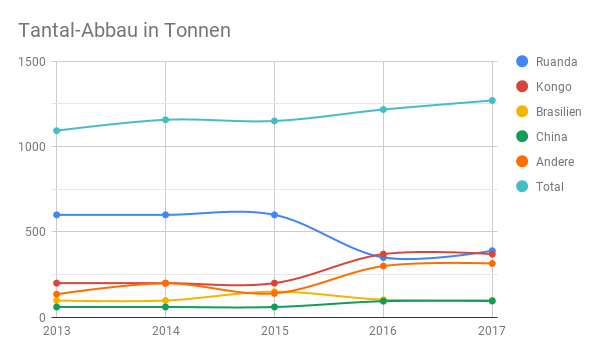
\includegraphics[width=0.8\textwidth]{tantal-abbau_in_tonnen}
    \caption{Weltweiter Tantal-Abbau mit den Top-4 Herkunftsländern. Quelle U.S. Geological Survey ~\cite{USGSMine8}}
    \label{fig:tantal_distribution}
\end{figure}

\subsection{Indikatoren}

Nachfolgend werden jeweils die einzelnen Indikatoren beschrieben, welche die
Basis für die gesellschaftliche Entwicklung der Nachhaltigkeit bilden.

\paragraph{Soziale Sicherheit}

Unter der sozialen Sicherheit werden Faktoren im Zusammenhang mit der
politischen Situation der Herkunftsländer zusammengefasst. Insbesondere der
Beitrag an die innenpolitische Stabilität des Landes trägt massgeblich zur
gesellschaftlichen Nachhaltigkeit bei.

\paragraph{Gesundheit}

Die Arbeitsverhältnisse in den Produktionsstätten für Tantal und die Folgen
der Umweltverschmutzung resultierend aus der Produktion auf die lokale
Bevölkerung sind die wichtigsten Aspekte für den Indikator Gesundheit.

\paragraph{Solidarität}

Der Indikator zur Solidarität umfasst das Bewusstsein der Konsumenten und
Märkte zur Herkunft und Produktion von Tantal.

\paragraph{Chancengleichheit}

Die Chancengleichheit umfasst das Verhältnis von Arbeitnehmer und
Arbeitnehmer in den Produktionsstätten, sowie den Einfluss auf die lokale
Bevölkerung.

\subsection{Bewertung}

\paragraph{2013} Gemäss dem U.S. Geological Survey stammen über 60\% der Mineralien für die
Tantalproduktion aus Zentralafrika ~\cite{USGSMine8}. Die Hälfte davon
wird in der Demokratischen Republik Kongo abgebaut, welches gemessen am Human Development Index als eines der ärmsten
Ländern der Welt gilt ~\cite{UNDProgramme2018}. Der Abbau von Mineralien im
Kongo wird von verschiedenen Konfliktparteien kontrolliert, welche wiederum
den Erlös aus den Minen zur Finanzierung des Konflikts nutzen. Aus diesem Grund
wird Tantal als Konfliktmineral klassifiziert ~\cite{doevenspeck2012konfliktmineralien}.
Gesellschaftlich hat dies einen negativen Einfluss auf die soziale
Sicherheit, da ein wesentlicher Teil des Gesamtvolumens aus Konfliktregionen
stammt und so zur Destabilisierung der betroffenen Regionen beiträgt \cite{Thespoil65}. 
Im Bezug auf die Gesundheit wirkt sich die Tantalgewinnung ebenfalls negativ aus, da die 
Produktionsstätten in den Konfliktgebieten ohne Rücksicht auf die Arbeiter und umliegende Umwelt
operieren.

Dem Indikator zur Solidarität wird eine positive Entwicklung zugeschrieben.
Dies zeigt sich an den zunehmenden Bemühungen die Einfuhr von Konfliktmineralien 
aufzudecken und zu regulieren. Als Beispiel sagt die EU-Verordnung zu Konfliktmineralien, 
welche im Jahr 2017 in Kraft getreten ist, dass alle Tantal-Importe in die EU die Standards zur nachhaltigen Beschaffung, definiert durch die OECD, erfüllen müssen ~\cite{europeancommission}. Die Effektivität solcher 
Massnahmen muss sich aber erst zeigen. So gibt es bereits eine Studie von Germanwatch zur EU-Verordnung, 
welche kritisiert, dass ``Unternehmen mit Scheinlösungen davonkommen könnten'' ~\cite{Governan35}.

In den Konfliktgebieten des Kongo und den Nachbarländern wie Ruanda ist der Abbau von 
Mineralien zur Produktion von Tantal eine wichtige Einkommensquelle für die lokale Bevölkerung
und eines der Haupt-Exportgüter der jeweiligen Länder ~\cite{OECProdu81}. Dies fliesst in
die Bewertung der Chancengleichheit ein, da ohne den Export dieser Mineralien die Verarmung
der Bevölkerung stark ansteigen würde ~\cite{DRCongo35}.

\paragraph{2035 bei anhaltendem Trend} Die Entwicklung der Konfliktregionen über die nächsten 20 Jahre
ist kaum vorherzusagen. Da die Demokratische Republik Kongo seit ihrer Unabhängigkeit 1960 von Gewaltausbrüchen geprägt ist und die Situation sich nicht zu bessern scheint ~\cite{Demokrat2}, wird für die 
Prognose angenommen, dass sich die Situation in den Konfliktgebieten nicht bedeutend bessern wird.
Die soziale Sicherheit wird für 2035 daher gleich bewertet wie 2013. 

Die zunehmende Anzahl an Massnahmen gegen Konfliktmineralien zeigt, dass die Solidarität und damit das Bewusstsein
der Konsumenten steigt ~\cite{Didthere42}. Dies führt zu einer besseren Bewertung als für 2013 und fliesst ebenfalls
positiv in den Indikator Gesundheit ein. Dies unter der Annahme, dass Massnahmen wie die EU-Verordnung Wirkung zeigen und einen nachhaltigen Abbau fördern. Ein positive Bewertung der Gesundheit wird dennoch nicht erreicht, da die Effektivität solcher Massnahmen von verschiedenen Seiten angezweifelt wird ~\cite{Demokrat2} ~\cite{TheEUCon25}. 

Die Chancengleichheit wird sich im Bezug auf die starke Nachfrage von Tantal in Ländern wie
Australien verbessern, wo auf Grund mangelnder Rentabilität ein Grossteil der Tantalproduktion  
eingestellt wurde ~\cite{Tantalum12}. Durch steigenden Preise werden die Minen wieder rentabel und 
so können zu Gunsten der Bevölkerung verlorene Arbeitsplätze wiederhergestellt werden.  

\paragraph{2035 mit Kondensatorenalternative} Ein Einbruch der Nachfrage nach Tantal wird die soziale Sicherheit in den Konfliktgebieten wahrscheinlich negativ beeinflussen. Es ist anzunehmen, dass sich der
Fokus auf die übrigen Mineralien wie Gold verstärken wird und bereits bestehende Konflikte um die Kontrolle der 
Minen fördert. Dies wird sich ebenfalls negativ auf die Gesundheit und Chancengleichheit auswirken. Der 
Verlust der Einkommensquelle der betroffenen Minenarbeiter, welche besonders in Konfliktgebieten darauf
angewiesen sind ~\cite{Obamasc19}, führt zu einer negativen Entwicklung der Chancengleichheit. 
Die Solidarität im Bezug auf die Tantalproduktion neutralisiert sich hingegen, da bei fehlender Nachfrage auch 
kein besonderes Bewusstsein für die Herkunft von Tantal vorhanden sein wird.  

\begin{table}[h]
    \centering
    \begin{tabular}{l|lll} & \textbf{2013} & \textbf{2035} &  \textbf{2035 mit Annahme} 
        \\ \hline Soziale Sicherheit    & 2  & 2  & 1
        \\ Gesundheit                   & 3  & 4  & 5
        \\ Solidarität                  & 6  & 7  & 5
        \\ Chancengleichheit            & 6  & 7  & 3
        \\ \hline \textbf{Endbewertung} & 4\(\frac{1}{4}\)  & 5  & 3\(\frac{1}{2}\)
    \end{tabular}
    \caption{Resultat gesellschaftliche Analyse}
\end{table}
